\def\currentRootFolder{chapter/modelOfIntegratedRate}
\def\currentFigureFolder{\currentRootFolder/fig}
\newacronym{standardmodel}{SM}{Standard Model of Particle Physics}
\newacronym{lep}{LEP}{Large Electron Positron Collider}
\newacronym{ssm}{SSM}{standard solar model}

\chapter{Model of the Integrated \texorpdfstring{$\upbeta$}{Beta}-Decay Rate Measured by KATRIN}
\label{sec:katrinExpIntSpecModel}
An analytic description for the electron rate measured by the \gls{fpd} can be derived. The derivation mostly follows \cite{Kleesiek2019, Groh2015, Kleesiek2014} or is extracted from current production code \cite{KATRINCOL2019}. The formulas are implemented in the so-called \gls{ssc} software framework.

\subsection{\texorpdfstring{$\upbeta$}{Beta} Decay Spectrum}
\begin{figure}
    \centering
    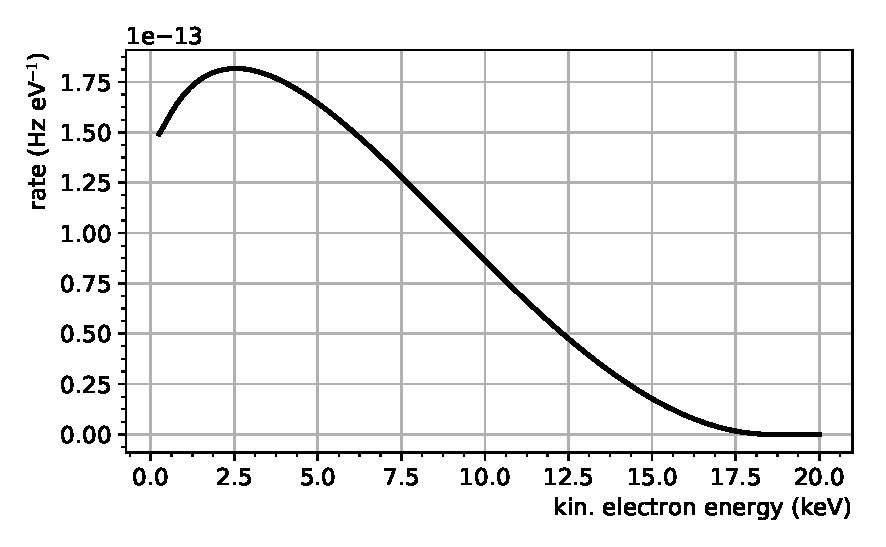
\includegraphics[width=\textwidth]{\currentFigureFolder/diffSpec.pdf}
    \xcaption{Tritium $\upbeta$ spectrum}{The $\upbeta$ decay spectrum of a tritium molecule}{as calculated by \gls{ssc}.}
    \label{fig:diffSpec}
\end{figure}
\label{sec:diffSpec}
In $\upbeta^-$ decay the released energy is distributed among the emitted electron and the anti-electron neutrino. The differential decay rate of a tritium molecule can be described using Fermi theory and Fermi's golden rule as
\begin{align}
    \label{eq:diffRate}
    \left(\diffRate\right) = &
    \frac{\fermiConst^2 \abs{V_\mathrm{ud}}^2}{2 \pi^3}
    \abs{\nucMatrixElement}^2 \cdot
    F(Z, E) \cdot 
    p(E+m_\elecIndex) \cdot 
    \sum_{f,i} P_f \abs{U_{\elecIndex i}}^2 \epsilon_f \sqrt{\epsilon_f^2-m_i^2} \cdot \thetaFunc(\epsilon_f-m_i)
\end{align}
It is depicted in figure \ref{fig:diffSpec}. Its constituents are the kinetic electron energy $E$;
the PMNS matrix $U$ \eqref{eq:PMNSmatrix}; the neutrino eigenmasses $m_i$ \eqref{eq:nuMassSquared};
the Fermi constant $\fermiConst$;
the up-down-quark-coupling given by the Cabibo angle $\theta_\mathrm{C}$
\begin{equation}
    V_\mathrm{ud} = \cos \theta_\mathrm{C} = 
    0.97425\pm0.00022;
\end{equation}
and the nuclear transition matrix element
\begin{equation}
    \nucMatrixElement = g_V^2+3g_A^2 \quad
    \text{with } g_v = 1 \quad
    \text{and} \quad g_A/g_V = -1.2646 \pm 0.0035
\end{equation}
which is independent of the electron's kinetic energy as the decay is super-allowed and given by the vector $g_V$ and axial vector $g_A$ coupling.

Furthermore, the Fermi function $F(Z,E)$ accounts for the Coulomb interaction between the outgoing electron and the daughter nucleus with atomic charge $Z=2$ which in its relativistic version can be approximated as
\begin{equation}
    F(Z,E) \approx \frac{2 \pi \eta}{1-\exp{2 \pi \eta}} \cdot R \\
\end{equation}
with Sommerfeld parameter $\eta = \alpha Z / \beta$, fine structure constant $\alpha$, relativistic velocity $\beta$ and a relativistic correction factor $R = 1.002037-0.001427\beta$.

The phase-space factor of the outgoing electron with momentum $p$ and mass $m_\elecIndex$ is given by the factor $p(E+m_\elecIndex)$.

The phase space factor of the emitted neutrino is described in dependence of the following quantities: total nuclear tritium decay energy $Q$ (mass difference of mother and daughter nucleus) corrected for the nucleus recoil $E_\mathrm{rec}$ also called endpoint of the $\upbeta$ spectrum
\begin{equation}
    \label{eq:endpoint}
    E_0 = Q-E_\mathrm{rec};
\end{equation}
the kinetic electron energy $E$ and the final state energy of the molecular system $V_f$. The probability that the molecular system is in a final state of energy $V_f$ after the decay is denoted by $P_f$. Then the energy of the neutrino reads 
\begin{equation}
    \epsilon_f = E_0 - E - V_f \fullstop
\end{equation}

The exited energy state $f$ is caused by vibration, rotation or electronic excitation of the decaying molecule. Details and tabulated values can e.g. be found in \cite{Bodine2015} and references therein.

The neutrino's momentum is $\sqrt{\epsilon_f^2-m^2_i}$, where $m_i$ denotes one of the neutrino eigenmasses. The complete phase space factor of the neutrino is a sum over all possible molecular final states labeled $f$ and neutrino eigenmasses labeled $i$.

Lastly, the Heavyside step function $\thetaFunc$ ensures a positive kinetic energy of the neutrino.

\subsection{Detector Counts}
The KATRIN detector counts electrons. The $\upbeta$ electrons are adiabatically guided from the \gls{wgts} to the detector by magnetic fields. The magnetic field lines are parallel to the beam line axis. The angle between the flight direction of a $\upbeta$ electron and the beam line axis towards the detector is denoted by the pitch angle $\theta \in [\SI{0}{\degree}, \SI{180}{\degree}]$. The starting position of an $\upbeta$ electron is denoted by its 1-dimensional coordinate along the beam line axis $\zSource$. 

KATRIN measures an integrated $\upbeta$ spectrum. In other words, the detector counts electrons of kinetic energy $\Esource$ above a threshold, the so-called retarding energy $qU$. The integrated $\upbeta$ spectrum can be scanned by varying $qU$.

A $\upbeta$ electron emitted in the \gls{wgts} reaches the detector with a probability modeled by the so-called response function $R$ (see section \ref{sec:response}). $R$ depends on the experimental settings (such as the electromagnetic fields and the gas dynamics) and especially on the retarding energy $qU$. Here, $R$ denotes the transmission probability for a $\upbeta$ electron of a fixed starting kinetic energy $\Esource$, starting position $\zSource$ and starting pitch angle $\thetaSource$. The probability of a $\upbeta$ electron for being counted when reaching the detector is denoted by the detection efficiency $\detEff$. Furthermore, the number of tritium molecules in the \gls{wgts} in a small area around the coordinate $z$ is denoted by $\d N_T(z)$. 

Then, the measured integrated rate is expressed as integral from the threshold energy $qU$ to the endpoint energy $E_0$ \eqref{eq:endpoint} over the differential rate $\d \Gamma / \d \Esource$ \eqref{eq:diffRate} weighted with the probability given by $R$ as
\begin{equation}
\label{eq:rateDependingOnstartingValues}
\Gamma(qU, \zSource, \thetaSource) = 
\detEff \cdot
\d N_T(\zSource) \cdot
\int_{qU}^{E_0} 
    \left(\frac{\d \Gamma(\Esource)}{\d \Esource}\right) \cdot 
    R(\Esource, qU, \zSource, \thetaSource) 
\d \Esource
\comma
\end{equation}
which eventually leads to $\upbeta$ electron counts by multiplication with the measurement time $t(qU)$ at a retarding energy $qU$
\begin{equation}
    \label{eq:countsDependingOnPositionAndPitchAngle}
    N(qU, \zSource, \thetaSource) = \Gamma(qU, \zSource, \thetaSource) \cdot t(qU)
    \fullstop
\end{equation}

\subsection{Discretization of the \glsentryshort{wgts} Volume}
\label{sec:sourceDiscretization}
The counts $N$ \eqref{eq:countsDependingOnPositionAndPitchAngle} are given for $\upbeta$ electrons of a fixed starting position $\zSource$.
All starting positions $\zSource \in [-L/2, +L/2]$ within the \gls{wgts} of length $L$ contribute to the total count rate at the detector. Integrating along the beam axis accounts for this
\begin{equation}
    N(qU, \thetaSource) = \int_{-L/2}^{+L/2} \frac{\d N(qU, \thetaSource, \zSource)}{\d \zSource} \d \zSource
\end{equation}
Numerically, the same result can be obtained by a sufficiently fine discretization of the \gls{wgts} volume into $S$ slices. The counts $N$ \eqref{eq:countsDependingOnPositionAndPitchAngle} are adapted accordingly to account for discrete starting $\upbeta$ electron positions $\zSource^j$
\begin{equation}
    N(qU, \thetaSource, \zSource) \rightarrow N^j(qU, \thetaSource,\zSource^j) \equiv N^j(qU, \thetaSource) \fullstop
\end{equation}
Then, the total counts read
\begin{equation}
    \label{eq:nonAveragedCounts}
    N(qU, \thetaSource) = \sum_{j=1}^S N^j(qU, \thetaSource) \fullstop
\end{equation}
Within this chapter, from here forth all quantities that are subject to discretization will be labeled with an upper index $j$. The discretization especially propagates to the response function $R \rightarrow R^j$ and its constituents.

\subsection{Magnetic Bottle Effect}
The $\upbeta$ electrons are adiabatically guided to the detector by magnetic fields. The magnetic field strength at the starting position of a $\upbeta$ electron in the \gls{wgts} is denoted by $\Bsource$. The maximum magnetic field strength along the beam line is denoted by $\Bmax$. As $\Bsource<\Bmax$ $\upbeta$ electrons travelling downstream to the detector are subject to the magnetic bottle effect. They get reflected and travel upstream to the rear wall if their starting pitch angle $\thetaSource$ surpasses $\thetaMax^j$ with
\begin{equation}
    \label{eq:thetaMax}
    \sin\thetaMax^j = \sqrt{\frac{\Bsource}{\Bmax}} \fullstop
\end{equation}
(Its KATRIN design value is $\thetaMax\approx \SI{51}{\degree}$.) A cutting angle $\thetaMax^j$ is beneficial because the greater the emission angle of a $\upbeta$ electron the larger the distance it travels in the \gls{wgts} and the more it is subject to energy losses such as scattering or synchrotron radiation.

\subsection{Scattering Probabilities}
\label{sec:scatProbs}
The probability for a $\upbeta$ electron to reach the detector (the response function $R^j$) depends on the scattering probabilities $P_l$ ($l \in \NN$). $P_l$ denotes the probability of an electron to scatter $l$ times when travelling through the \gls{wgts}. $P_l$ depends on the starting position $\zSource$ of a $\upbeta$ electron in the \gls{wgts} as well as on its starting pitch angle $\thetaSource$. The expected scattering count for a $\upbeta$ electron when travelling through the \gls{wgts} is the product of the line density $\lambda$ the electron passes through and the scattering cross section $\sigma$
\begin{equation}
    \label{eq:expectedScatteringCount}
    \mu(\zSource, \thetaSource) = \lambda(\zSource,\thetaSource) \sigma \fullstop
\end{equation}
The electron moves on a spiral due to its cyclotron motion. Therefore, when traveling an infinitesimal distance $\d z$ in $z$-direction, it travels a total distance of
\begin{equation}
    \label{eq:infinitesimalElecPath}
    \d s = \frac{1}{\cos\thetaSource} \d z \fullstop
\end{equation}
The line density $\lambda$ can be expressed as a line integral over the gas density $\rho$ along the electrons path $\varphi$
\begin{equation}
    \label{eq:lambdaPath}
    \lambda(\zSource,\thetaSource) = \int_{\varphi} \rho(\Vec{r})\d s
    \fullstop
\end{equation}
Assuming that the gas density $\rho$ only depends on the $z$-position along the beam line and vanishes for $z>L/2$ (beyond the \gls{wgts}) equation (\ref{eq:lambdaPath}) becomes
\begin{equation}
    \label{eq:lambdaPathIntegral}
    \lambda(\zSource,\thetaSource) = \frac{1}{\cos\thetaSource}\int_{\zSource}^{L/2} \rho(z)\d z \fullstop
\end{equation}
Hence, the expected scattering count (\ref{eq:expectedScatteringCount}) becomes
\begin{equation}
    \label{eq:expectedScatRate}
    \mu(\zSource, \thetaSource) = \frac{\sigma}{\cos\thetaSource}\int_{\zSource}^{L/2} \rho(z)\d z \fullstop
\end{equation}
The scattering process fulfills the conditions of a Poisson process, namely scattering once does quasi not influence the probability of an electron to scatter again; the expected scattering count $\mu$ \eqref{eq:expectedScatRate} stays quasi constant; and it is unlikely for two scatterings to happen within a short distance. Thus, the probability for $l$-fold scattering can be expressed as a Poisson distribution
\begin{equation}
    \label{eq:scatProbs}
    P_l(\zSource, \thetaSource) = 
    \frac{
        \mu(\zSource, \thetaSource)^l
    }{l!}
    \mathrm{e}^{-\mu(\zSource, \thetaSource)} \fullstop
\end{equation}
\paragraph{Discretization of the \gls{wgts} volume}
In the discretized case the \gls{wgts} volume is divided into $S$ slices indexed by $k$ with an average gas density $\bar{\rho}^k$. A slice $k$ starts at position $Z_s^k$ and ends at position $Z_e^k$ with a width of $W^k=Z_e^k-Z_s^k$. For $\upbeta$ electrons that start at a position $z$ within slice $j$ the expected scattering count \eqref{eq:expectedScatteringCount} becomes
\begin{equation}
\label{eq:nonAveragedExpectedScatCount}
    \mu(\zSource, \thetaSource) \rightarrow 
    \mu^j(z, \thetaSource) =
    \frac{\sigma}{\cos\thetaSource}
    \underbrace{
        (Z_e^j-z) \bar{\rho}^j
        \vphantom{\sum_{k=j+1}^{S}}
    }_{(*)}
    \underbrace{\sum_{k=j+1}^{S} \bar{\rho}^k W^k}_{(**)}
    \fullstop
\end{equation}
The gas column density in front of a $\upbeta$ electron is split in two parts: the slice of its \mbox{origin $(*)$} and all slices downstream \mbox{$(**)$}. 

The Poisson distribution is formed for the expected scattering count $\mu^j$ \eqref{eq:nonAveragedExpectedScatCount} and averaged over all starting positions within the slice $j$ which yields the discretized scattering probabilities
\begin{equation}
    \label{eq:nonAveragedScatProbs}
    P^j_l(\thetaSource) = 
    \frac{1}{W^j}
    \int_{Z_s^j}^{Z_e^j}
        \frac{
            \left(\mu^j(z,\thetaSource)\right)^l
        }{l!}
        \mathrm{e}^{-\mu^j(z,\thetaSource)}
    \d z
    \fullstop
\end{equation}


\subsection{\glsentryshort{mace} Principle and Transmission Function}
\label{sec:mace}
\begin{figure}[t]
	\inputpdftex{\currentFigureFolder/mace}
	\xcaption{Scheme of the KATRIN main spectrometer and the \glsentryshort{mace} filter principle.}{
		Scheme of the KATRIN main spectrometer and the \glsentryfull{mace} filter principle.}{
		The {KATRIN} design magnetic field settings are
		$\Bps=\SI{4.5}{T}$, 
		$\Bsource=\SI{3.6}{T}$, 
		$\Bmax=\SI{6.0}{T}$, 
		$B_\mathrm{D}=\SI{3.6}{T}$, 
		$\Bana\approx\SI{3e-4}{T}$. $\Vec{E}$ denotes the magnetic field regulated by the retarding potential $U$ that reaches its maximum $U_\mathrm{a} = U$ at the analyzing plane. (Adapted from \cite{SeitzM2019})
	}
	\label{fig:mace}
\end{figure}

The spectrometers of KATRIN follow the \glsentryfull{mace} principle. Figure \ref{fig:mace} shows a corresponding sketch. The main spectrometer is a vacuum vessel with a downstream magnet of strength $\Bps$ and an upstream magnet of strength $\Bpinch$ making electrons form a magnetic flux tube. In the case of KATRIN the fluxtube begins in the \gls{sts} with a magnetic field strength of $\Bsource$. In other words, the spectroscopic properties are not solely determined by the spectrometer vessel, but also by the \gls{sts}. The minimum magnetic field strength $\Bmin = \Bana$ is reached at the so-called analyzing plane in the vessel center. Electrons entering the vessel perform cyclotron motions around the magnetic field lines. Their total kinetic energy $\Esource$ is split into a longitudinal component $E_\parallel$ along the beam axis and a transverse component $E_\bot$
\begin{equation}
    \label{eq:totalKinElecEnergy}
    \Esource = E_\parallel + E_\bot \fullstop
\end{equation}
In the non-relativistic and adiabatic approximation the transverse component can be expressed by the magnetic field strength $B$ and the electron's magnetic moment $\mu$ respectively its charge $q=e$, its mass $m_\elecIndex$ and angular momentum $L$.
\begin{equation}
    E_\bot = - \mu B = \frac{e}{2 m_\elecIndex}LB \fullstop
\end{equation}
Adiabaticity conserves angular momentum $L$ and the total energy of the electron $\Esource$. Hence, when the magnetic field strength $B$ decreases to $\Bana=\Bmin$ in the analyzing plane, the transverse component of the electron's energy $E_\bot$ decreases likewise and transforms to longitudinal energy $E_\parallel$. Additionally, a retarding voltage barrier is applied along the beam axis, reaching its maximum $U$ at the analyzing plane and dropping of towards the source and the detector. 
In order to pass through the filter, electrons need a total kinetic energy $\Esource$ greater than the transmission energy $\Etrans$ that depends on their starting potential $\Usource$, their starting pitch angle $\thetaSource$ and starting Lorentz factor $\gammaSource$
\begin{equation}
    \label{eq:transmissionEnergy}
    \Etrans = 
    \frac{
        q(U-\Usource)
    }{
        1-\sin^2\thetaSource \frac{\Bana}{\Bsource} \frac{\gammaSource+1}{2}
    }
    \fullstop
\end{equation}
For ease of notation, the dependency on $\Bsource$, $\Bana$ and $\Usource$ is left implicit. Note further that the right hand side of \eqref{eq:transmissionEnergy} also depends on the starting energy of a $\upbeta$ electron as it depends on $\gammaSource$.

Then, the probability for an electron to pass through a \gls{mace} filter, the so-called transmission function, can be written as
\begin{equation}
    \label{eq:transmissionWithConditionOnEnergy}
    \mathcal{T}^j(\Esource, qU, \thetaSource) =
    \begin{cases}
    1 & \text{if } \Esource > \Etrans \\
    0 & \text{otherwise} 
    \end{cases}
    \fullstop
\end{equation}

The transmission condition for the energy $\Esource > \Etrans$ can be reformulated to a condition for the pitch angle $\thetaSource^j$
\begin{align}
    \label{eq:transmissionPitchAngle}
    &\Esource > \Etrans \\
    \Leftrightarrow \quad
    & \thetaSource < \thetaTrans
    \coloneqq
    \arcsin
    \left(\sqrt{
        \frac{\Esource-q(U-\Usource)}{\Esource} 
        \frac{\Bana}{\Bsource}
        \frac{\gammaSource+1}{2}
    }\right)
\end{align}
This allows to rewrite the transmission function \eqref{eq:transmissionWithConditionOnEnergy} as
\begin{equation}
    \label{eq:transmission}
    \mathcal{T}^j(\Esource, qU, \thetaSource) =
    \begin{cases}
    1 & \text{if } \thetaSource > \thetaTrans \\
    0 & \text{otherwise} 
    \end{cases}
    \fullstop
\end{equation}

\subsection{Response Function}
\label{sec:response}
The so-called response function denotes the probability of a $\upbeta$ electron emitted in the \gls{wgts} with starting energy $\Esource$ and pitch angle $\thetaSource$ to reach the detector when a retarding voltage of $U$ is applied to the spectrometer. In addition to the transmission function $\mathcal{T}^j$ \eqref{eq:transmissionPitchAngle} it incorporates the energy loss $\epsilon$ of the $\upbeta$ electrons due to scattering in the gas in the \gls{wgts}. If up to $N$-fold scattering is considered, the response function reads
\begin{equation}
    \label{eq:nonAveragedResponse}
    R^j(\Esource, qU, \thetaSource) = 
    \int_0^{\Esource}
        \sum_{l=1}^{N}
            \mathcal{T}^j(\Esource-\epsilon, qU, \thetaSource) \cdot
            P^j_l(\thetaSource) \cdot f_l(\epsilon)
    \d \epsilon
    \fullstop
\end{equation}
Here, $P^j_l$ \eqref{eq:nonAveragedScatProbs} denotes the probability of a $\upbeta$ electron to scatter $l$ times when travelling through the \gls{wgts}. $f_l(\epsilon)$ is the so-called energy loss function. It denotes the probability for $\upbeta$ electrons to loose the energy $\epsilon$ when scattering $l$ times. For no scattering the Dirac delta function is used
\begin{equation}
    f_0(\epsilon) = \delta(\epsilon) \fullstop
\end{equation}
For $1$-fold scattering $f_1$ is denoted without index $f_1 = f$. For $l>1$ and $l$-fold scattering $f_l$ is the $l$-fold convolution of $f$ with itself
\begin{equation}
    f_l(\epsilon) = \Conv_{i=1}^{l} f(\epsilon)
\end{equation}
where $\conv$ denotes the convolution
\begin{equation}
    (f \conv f)(\epsilon) = \int_{0}^{\infty}  f(\epsilon-\epsilon^\prime)f(\epsilon^\prime) \d \epsilon^\prime \fullstop 
\end{equation}

\subsection{Energy Loss Function}
\label{sec:eloss}
The response function \eqref{eq:nonAveragedResponse} depends on the energy loss function $f$. $f(\epsilon)$ denotes the probability of a $\upbeta$ electron to loose the energy $\epsilon$ when scattering once on a gas molecule. A review of different models for $f$ can e.g. be found in \cite{Trost2019}. E.g. a phenomenological model fitted to data was established by the Troitsk experiment for tritium \cite{Aseev2000} as well as for deuterium and hydrogen molecules \cite{Abdurashitov2017}. Currently a corresponding  modeling effort is made based on data taken by KATRIN. Details will be discussed in section \ref{sec:elossSensitivity}.

\subsection{Distribution of Pitch Angles}
\label{sec:pitchAngleAveraging}
The detected counts $N$ (\ref{eq:nonAveragedCounts}) are given for a fixed starting pitch angle $\thetaSource$ of $\upbeta$ electrons which motivates to average over pitch angles. Any function $g(\thetaSource)$ depending on a fixed pitch angle $\thetaSource$ can be averaged given the distribution $\omega(\thetaSource)$ of $\thetaSource$ and its maximum value $\thetaMax^j$ \eqref{eq:thetaMax} as
\begin{equation}
    \label{eq:pitchAngleAveraging}
    \langle g(\thetaSource) \rangle \equiv \bar{g} =  
    \frac{
        \int_{0}^{\thetaMax^j} 
            \omega(\thetaSource)
            g(\thetaSource)
        \d \thetaSource   
    }{
        \int_{0}^{\thetaMax^j} 
            \omega(\thetaSource)
        \d \thetaSource 
    } \fullstop
\end{equation}
An isotropic $\upbeta$ electron emission by a tritium molecule into the unit sphere, meaning all combinations of spherical emission angles $(\varphi, \vartheta=\thetaSource)$ are equally likely, yields as distribution for their starting pitch angle
\begin{align}
    \omega(\thetaSource) &= \sin\thetaSource \\
    \int_{0}^{\thetaMax^j} 
            \omega(\thetaSource)
        \d \thetaSource 
    &= \frac{1}{1-\cos\thetaMax^j}
    \fullstop
\end{align}

\paragraph{Scattering Probabilities}
Averaging the scattering probabilities $P_l^j$ \eqref{eq:nonAveragedScatProbs} yields
\begin{equation}
    \label{eq:averagedScatProbs}
        \bar{P}_l^j = \frac{1}{1-\cos\thetaMax^j} \int_{0}^{\thetaMax^j} P_l^j(\thetaSource) \sin\thetaSource \d \thetaSource \fullstop
\end{equation}
This expression is helpful when averaging the detected counts $N$ \eqref{eq:nonAveragedCounts} and bringing the corresponding averaged response function in a demonstrative form as shown below.

\paragraph{Counts and Response Function}
\begin{figure}
    \centering
    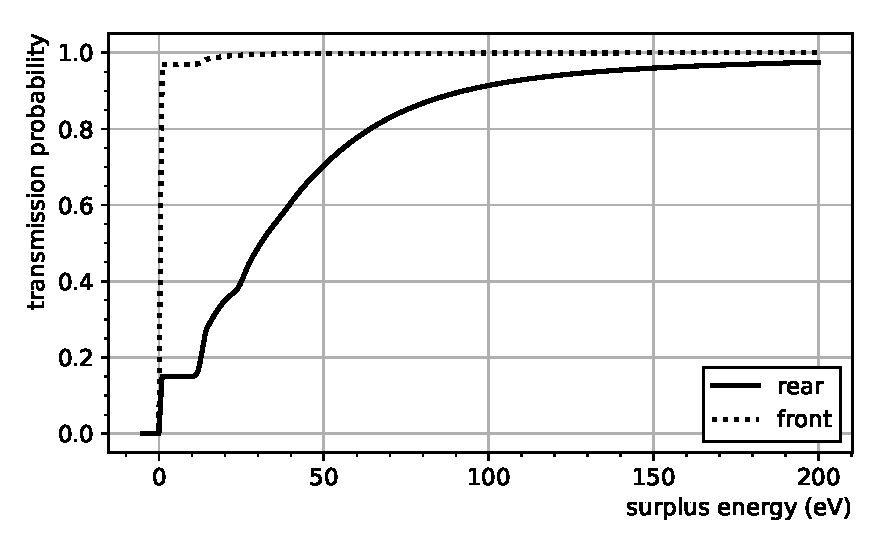
\includegraphics[width=\textwidth]{\currentFigureFolder/response.pdf}
    \xcaption{KATRIN response function}{The response function}{as calculated by \gls{ssc}. The surplus energy denotes the difference between the starting kinetic energy $\Esource$ of a $\upbeta$ electron and the retarding energy $qU$. The response function $\bar{R}^j$ \eqref{eq:SSCresponse} is depicted for electrons starting at the rear and front of the \gls{wgts}.}
    \label{fig:response}
\end{figure}
The detected counts $N$ \eqref{eq:nonAveragedCounts} depend on the starting pitch angle $\thetaSource$ of the $\upbeta$ electrons. They have to be averaged over $\thetaSource$. The corresponding integral can be swapped with the sum over the \gls{wgts} slices and the integral over the energy and propagates to the response term
\begin{align}
\label{eq:SSCcounts}
\bar{N}(qU) \propto \sum_{j=1}^S N_T^j
\int_{qU}^{E_0}
    \left(\frac{\d \Gamma(\Esource)}{ \d \Esource}\right) \cdot
    \frac{1}{1-\cos\thetaMax^j}
    \int_{0}^{\thetaMax^j}
        R^j(\Esource, qU, \thetaSource) 
        \sin\thetaSource \d \thetaSource
\d \Esource
\fullstop
\end{align}
Here $N_T^j$ denotes the number of tritium molecules in a \gls{wgts} slice $j$. The response function $R^j$ (\ref{eq:nonAveragedResponse}) can be averaged as
\begin{equation}
\begin{split}
    \bar{R}^j(\Esource,qU) &= 
    \frac{1}{1-\cos\thetaMax^j}
    \int_{0}^{\thetaMax^j}
        R^j(\Esource, qU, \thetaSource) 
    \sin\thetaSource \d \thetaSource \\ &=
    \int_0^{\Esource}
        \sum_{l=1}^{N}
            \frac{1}{1-\cos\thetaMax^j}
            \int_{0}^{\thetaMax^j}
            \mathcal{T}^j(\Esource-\epsilon, qU, \thetaSource) \cdot
            P^j_l(\thetaSource)
            \sin\thetaSource \d \thetaSource
            f_l(\epsilon)
    \d \epsilon
    \fullstop
\end{split}
\end{equation}
The transmission function $\mathcal{T}^j$ \eqref{eq:transmission} is a step function. Assuming that $\thetaMax^j$ \eqref{eq:thetaMax} is always greater than the transmission angle $\thetaTransPure$ \eqref{eq:transmissionPitchAngle}, the upper integral boundary changes which yields the averaged response function
\begin{equation}
    \label{eq:slimResponse}
    \bar{R}^j(\Esource, qU) =
    \int_0^{\Esource}
        \sum_{l=1}^{N}
            \int_{0}^{\thetaTransPure(\Esource-\epsilon, qU)}
            \frac{
                \sin\thetaSource \cdot P^j_l(\thetaSource)
            }{
                1-\cos\thetaMax^j
            }
            \d \thetaSource
            f_l(\epsilon)
    \d \epsilon
    \fullstop
\end{equation}
The averaged response function $\bar{R}^j$ is depicted in figure \ref{fig:response}. Its formula \eqref{eq:slimResponse} can be rewritten to match the form of the formula for the non-averaged response function \mbox{$R^j$ \eqref{eq:nonAveragedResponse}}. Therefore, the averaged scattering probabilities $\bar{P}^j_l$ \eqref{eq:averagedScatProbs} are used and the factor $1 = \bar{P}^j_l / \bar{P}^j_l$ is inserted in equation \eqref{eq:slimResponse}:
\begin{align}
    \label{eq:implementedResponse}
    \bar{R}^j(\Esource, qU) &=
    \int_0^{\Esource}
        \sum_{l=1}^{N}
            \underbrace{
                \int_{0}^{\thetaTransPure(\Esource-\epsilon, qU)}
                \frac{
                    \sin\thetaSource \cdot P^j_l(\thetaSource)
                }{
                    (1-\cos\thetaMax^j) \cdot \bar{P}^j_l
                }
                \d \thetaSource
            }_{
                T^{j,\star}(\Esource-\epsilon, qU)
            } \cdot 
            \bar{P}^j_l \cdot
            f_l(\epsilon)
    \d \epsilon \\ &=
    \int_0^{\Esource}
        \sum_{l=1}^{N}
            T^{j,\star}(\Esource-\epsilon, qU) \cdot 
            \bar{P}^j_l \cdot
            f_l(\epsilon)
    \d \epsilon
    \label{eq:SSCresponse}
    \fullstop
\end{align}
Note that the non-averaged response function $R^j$ \eqref{eq:nonAveragedResponse} has the same form as the averaged one $\bar{R}^j$ \eqref{eq:SSCresponse} if the non-averaged transmission function $\mathcal{T}^j$ \eqref{eq:transmission} is replaced by the modified transmission function $T^{j,\star}$ and the non-averaged scattering probabilities $P^j_l$ (\ref{eq:scatProbs}) by the averaged ones $\bar{P}^j_l$ \eqref{eq:averagedScatProbs}.

Note further that albeit equation (\ref{eq:slimResponse}) and equation (\ref{eq:SSCresponse}) are analytically equal, they are not equal implementation-wise. Currently the implementation of the response function follows equation (\ref{eq:SSCresponse}). One one hand, equation (\ref{eq:slimResponse}) is more ``light-weight'' as it does not use the averaged scattering probabilities. In the future it might be beneficial to alter the implementation to simplify the program structure and cut down on the number of calculations. On the other hand, equation \eqref{eq:implementedResponse} allows the exchange of implementations for the transmission function whereas equation \eqref{eq:slimResponse} only allows to exchange the implementation of the response function as a whole.

\subsection{Reconciliation}
The predicted counts for a retarding energy of $qU$ when measuring a duration $t(qU)$ are
\begin{equation}
	\label{eq:countsSCCFinal}
	\bar{N}(qU) = t(qU) \cdot \detEff \cdot \left(
		\As \cdot
		 \sum_{j}
			N_T^j \cdot
			\int_{qU}^{E_0} 
				\left(\frac{\d \Gamma(\Esource)}{ \d \Esource}\right) \cdot 
				\bar{R}^j(\Esource, qU) 
			\d \Esource +
			\Rbg
		\right)
	\fullstop
\end{equation}
Here, $\As=1$ is a normalization factor, $\detEff \in [0,1]$ is the detector efficiency, the sum goes over all source slices, $N_T^j$ is the number of tritium molecules in the $j$th source slice, $\left(\d \Gamma(\Esource) / \d \Esource \right)$ is the differential rate from \eqref{eq:diffRate}, $\bar{R}^j(\Esource, qU)$ is the response function from \eqref{eq:SSCresponse} and $\Rbg$ is the rate of background events.

\subsection{Amendments}
Equation \eqref{eq:countsSCCFinal} is a scaffold for an analytic model of the counts measured by the KATRIN detector. Modifications of isolated terms can consider further effects. Selected examples are:
\begin{itemize}
    \item \textbf{Doppler effect:} Gas flow and temperature move the tritium molecules and hence, smear the kinetic energy distribution of $\upbeta$ electrons. This can be modelled by convolving the differential rate $\d \Gamma / \d E$ \eqref{eq:diffRate} with a Maxwellian distribution or by applying corrections to the final energy states of the decaying molecules.
    \item \textbf{Plasma potential:} Space charges, respectively a plasma, forms within the \gls{wgts} due to the tritium decay. Electrons passing through space charges might either gain or loose energy. In a segmented \gls{wgts} volume, this is implemented by using an effective retarding energy corrected for the plasma potential $V^j$ in the slice $j$
    \begin{equation}
        qU \rightarrow qU^j_\mathrm{eff} = qU - V^j
    \end{equation} 
    when calculating the response function $\bar{R}^j$ \eqref{eq:SSCresponse}. Note that this is equivalent to using the starting potential $\Usource$ in the transmission energy $\EtransPure$ \eqref{eq:transmissionEnergy}.
    \item \textbf{Further discretization of the \gls{wgts} volume:} The \gls{ssc} software allows to discretize the \gls{wgts} not only into slices, but also to subdivide the slices further into rings and the rings into segments. This enables an arbitrary spacial binning for \gls{wgts} properties such as the magnetic field or gas density. Then, additionally, the retarding energy $qU \rightarrow qU^j$, the maximum magnetic field strength  along the beam line $\Bmax \rightarrow \Bmax^j$, the magnetic field strength in the analyzing plane $\Bana \rightarrow \Bana^j$ and the detector efficiency $\epsilon_\mathrm{det} \rightarrow \epsilon_\mathrm{det}^j$ become subject to discretization because they exhibit a radial dependency. Furthermore, the \gls{wgts} can be subdivided into volumes that map onto a specific detector pixel due to magnetic guidance. This enables pixel-wise modelling of electron counts.
\end{itemize}

\def\currentRootFolder{chapter/modelOfIntegratedRate/neutrinoMassMeasurement}
\def\currentFigureFolder{\currentRootFolder/fig}
\newcommand{\elecIndex}{\mathrm{e}}

\newcommand{\Bsource}{B^j_\mathrm{S}}
\newcommand{\BsourceAvg}{B_\mathrm{S}}
\newcommand{\zSource}{z_\mathrm{S}}
\newcommand{\thetaSource}{\theta_\mathrm{S}}
\newcommand{\thetaSourceAvg}{\theta_\mathrm{S}}
\newcommand{\Esource}{E_\mathrm{S}}
\newcommand{\Usource}{U^j_\mathrm{S}}
\newcommand{\gammaSource}{\gamma_\mathrm{S}}


\newcommand{\Bps}{B_\mathrm{PS2}}
\newcommand{\Bana}{B_\mathrm{A}}
\newcommand{\Bpinch}{B_\mathrm{P}}
\newcommand{\Bmax}{B_\mathrm{max}}
\newcommand{\Bmin}{B_\mathrm{min}}

\newcommand{\thetaMax}{\theta_\mathrm{max}}
\newcommand{\Esur}{E_\mathrm{sur}}
\newcommand{\detEff}{\epsilon_\mathrm{det}}
\newcommand{\macefilterwidth}{\Delta \mathcal{E}^j(\thetaS^j)}

\newcommand{\EtransPure}{E^j_\mathrm{tr}}
\newcommand{\Etrans}{\EtransPure(qU,\Esource,\thetaSource)}
\newcommand{\thetaTransPure}{\theta^j_\mathrm{tr}}
\newcommand{\thetaTrans}{\thetaTransPure(\Esource,qU)}

\newcommand{\As}{A_\mathrm{S}}
\newcommand{\Rbg}{R_\mathrm{bg}}


\newacronym{standardmodel}{SM}{Standard Model of Particle Physics}
\newacronym{lep}{LEP}{Large Electron Positron Collider}
\newacronym{ssm}{SSM}{standard solar model}

\section{A KATRIN Neutrino Mass Measurement}
\label{sec:katrinExpNuMassMeasurement}
\todo{Introduction}
The predicted counts for a retarding energy of $qU$ when measuring a duration $t(qU)$ are
\begin{equation}
\label{eq:intSpecModelCountsFinal}
\bar{N}(qU) = t(qU) \cdot \detEff \cdot \left(
\As \cdot
\sum_{j}
N_T^j \cdot
\int_{qU}^{E_0} 
\left(\frac{\d \Gamma(\Esource)}{ \d \Esource}\right) \cdot 
\bar{R}^j(\Esource, qU) 
\d \Esource +
\Rbg
\right)
\fullstop
\end{equation}
Here, $\As=1$ is a normalization factor, $\detEff \in [0,1]$ is the detector efficiency \todo{reference KATRIN chapter}, the sum goes over all source slices with label $j$, $N_T^j$ is the number of tritium molecules in the $j$th source slice, $\left(\d \Gamma(\Esource) / \d \Esource \right)$ is the differential rate from \eqref{eq:intSpecModelDiffSpec}, $\bar{R}^j(\Esource, qU)$ is the response function from \eqref{eq:} and $\Rbg$ is the rate of background events.

KATRIN measures electron counts as described in \eqref{eq:countsSCCFinal} at a set of retarding energies ${qU_i}$. How much measurement time $t(qU_i)$ is attributed to a certain retarding energy is called a \gls{mtd}. The \gls{mtd} influences the experiment's sensitivity to the neutrino mass. An optimal \gls{mtd} balances the following aspects:
\begin{enumerate}
	\item Some measurement time has to be attributed to retarding energies beyond the endpoint of the spectrum to determine the background rate. The optimal duration depends on the background rate.
	\item The shape of the integral tritium $\upbeta$ spectrum depends the strongest on the neutrino mass near its endpoint $E_0$ \eqref{eq:endpoint}. \todo{Plot!}
	\item Measurements deeper into the spectrum increase the count rate and hence, lower the statistical uncertainty due to Poisson statistics.
	\item The theoretical description of the integral tritium $\upbeta$ spectrum is optimized for the endpoint region. Deeper scans introduce modeling uncertainties.
\end{enumerate}
The KATRIN Design Report \cite{Angrik:2005ep} suggests 5 \gls{mtd}s for different measurement ranges $[E_0-\alpha\;\SI{}{eV}, E_0 + \SI{5}{eV}]$ with $\alpha \in \{20, 25, 30, 40, 50\}$ and the conclusion that $\alpha=30$ yields the best sensitivity to the neutrino mass. Furthermore, searches for sterile neutrinos at the keV-scale would require deeper scans~\cite{Kleesiek2014}. Several measurement campaigns were already conducted. The \gls{ft} commissioning campaign successfully proved the apparatus functioning. The corresponding \gls{mtd} covered a range starting at $\sim E_0-\SI{1.6}{keV}$. The \gls{knm1} campaign is evaluated during the writing of this thesis. It set out to establish an unprecedented limit on the neutrino mass by $\upbeta$-decay measurements. Its \gls{mtd} starts at $\sim E_0-\SI{90}{eV}$.